\chapter{Context}\label{sec:chap:3}
Exercise is something that constitutes a major aspect of a person’s life from cross country running to weight training, and everything in between. The problem is that for many activities even though we now have access to massive amounts of information thanks to having access to the internet in the palm of our hands, it is still a pain to search for how to correctly exercise our bodies and what is best to efficiently do so. This makes something that improves our health to something that may cause injury.\\

 
This is reflected every year in gyms, where every New Year there is an influx of people that join and after a few weeks they end up abandoning their New Year’s resolution. In America 13 \% of all New Year’s resolutions are related to losing weight and exercising, making it the most common resolution. With google trends, that shows what users search for, we can corroborate these results with the interest people have of subjects like exercising and weight loss were there are major spikes of interest at the beginning of every year that slowly dies of towards the end of the year.\cite{newyear}


\begin{center}
	\begin{figure}[h!]
		\centering
		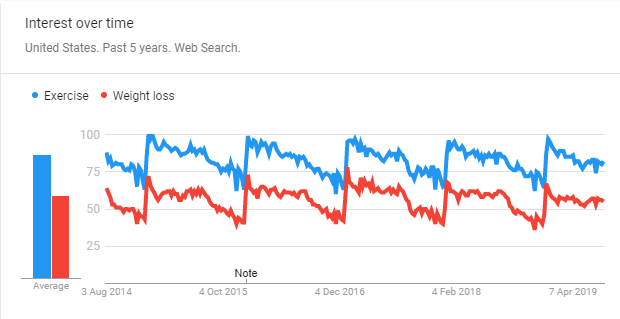
\includegraphics[scale=0.9]{./images/2-new-year-exercise}
		\caption{User Trends}
		\label{user-trends-gym}
	\end{figure}
\end{center}

Thanks to gym applications gaining popularity the amount of data gathered allows the creation of some interesting conclusions where in the following graph can be seen how many activity logs uploaded to Strava’s fitness app, this graph separates the different age groups which helps figure out which groups are more common to abandon and retake the gym after New Year. From the following graph older age groups have a higher tendency to start their resolutions as soon as possible, where younger age groups tend to have a smoother approach when starting their resolutions. What they have in common is that all groups show a decrease in activity logs towards the end of the year.\cite{newyear}\\

\begin{center}
	\begin{figure}[h!]
		\centering
		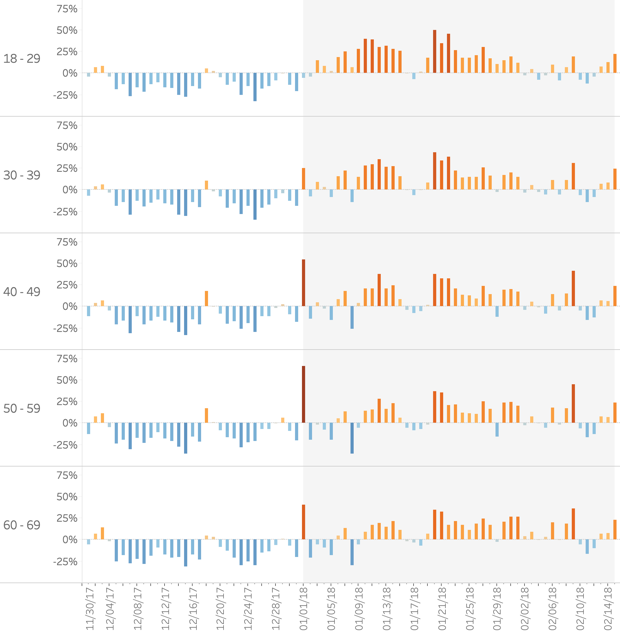
\includegraphics[scale=0.6]{./images/2-new-year-logs}
		\caption{User Activity Log Uploads}
		\label{user-logs-gym}
	\end{figure}
\end{center}

The conclusion of this analysis is that there is a motivation to get fit, but people have problems in maintaining their routines.  One of the reasons are unrealistic expectations where people want to tackle a big objective without being experienced or being disciplined, another of the reasons are boring workouts where people only do the exercises they have seen in films and don’t change their routine because they don’t have the knowledge to do so. Because of this and many other reasons the resolution to go to the gym quickly dies of.\cite{newyear_logs}\\

\section{Objectives}\label{sec:chap2_objectives}

The main objective is to have a functional virtual assistant that can provide the same help as normal personal trainers but at a much lower cost. This project will be a proof of concept with some limited functionality to see the viability of the product, the project will be focused on gym training.\\
The objective of the chatbot is to help users stay active, the way this will be accomplished is by making it easier for them to stay motivated and keep reaching their objectives. Reviewing the most common reasons people quit doing exercise comes down to unreasonable objectives and a lack of knowledge.\\

The following points reflect the main functionality the bot will have in it’s final form to help the user reach their goals:
\begin{itemize}
	\item {\textbf{Exercise table creation:}  One of the most time-consuming and boring things to do is prepare a routine to follow, there are applications that help out with this, but the idea for this project is to make the interaction more human-like, having the bot automatically generate tables based on what muscles have been trained and what muscles are not proportionate to the rest of the body. As this is a proof of concept and due to the time constraint of this project, the functionality that tracks what the user has exercised and the table creation will be limited.}
	\item {\textbf{Diets table creation:} Like what the above point talks about, the objective here is to make it easier for the user to know what to eat in order to reach their desired weight or to gain muscle mass. As some users may have different meal preferences, for the final product the chatbot can take food preferences in to account to provide different meals.}
	\item {\textbf{User tracking:} The objective is to track the user’s progress and see how close they are of fulfilling their goals, this will provide data on each user’s performance and how to further adapt their routines to make it easier to follow.}
	\item {\textbf{Motivate user regularly:} By checking how their training sessions are going and how well the users are progressing, motivate them with data on their progress and how close they are of achieving their goals.}
	\item {\textbf{Training sessions:} This objective would be an addition for future development as it requires a different architecture and it is still not technologically ready. The idea is to have a human-like voice speak while you complete your training sessions. The problem is making the voice human-like and the technology is not there yet. The idea of doing it written distracts the user by making the user use the phone more. }
	 
\end{itemize}	 
These objectives when completed will provide the user with enough tools to feel motivated and keep them using the application, where certain functionality may require being a premium member. This will fulfil the objective of making the application profitable, another way to increase profitability would be using ads related to health products the user can buy based on the chatbots recommendations, from protein shakes to measurement tools.

\section{Socioeconomic Environment}\label{sec:chap2_socio_frame}
\subsection{Social Impact}\label{sec:chap6_soc}

The social impact of this project is something that must be analyzed as this type of technology even though have been around for some time, at the pace it is evolving can soon cause them to truly seem human like. This is a problem or at least something that must be taken account as people don’t like to feel fooled, if we consider the impact Google Duplex has had since it launched, people where amazed and scared of the fact that the assistant used human behavior while talking like humming while it searched for information.\\

Other things to consider as a social impact would be the other way around, the vulnerability of chatbots, as it is a machine interacts with people it must be correctly designed to stop users from accessing privileged information or extracting information from the system. Another factor is the fact that some chatbots learn from interactions, if not careful these interactions may be racist or contain offensive content that may cause the chatbot to become a part of that it learns.\\

The positive impact of this project socially is the fact that when fully developed will provide a way for connecting with new people and make it easier for people to train without having to spend a large amount of money or time to learn how to do exercises correctly or what routes are better to run.\\

Another social impact of this project if it catches the user’s attention and use it regularly is that the health benefits of training will compensate indirectly with health issues caused by obesity or heart problems.


\subsection{Economic Impact}\label{sec:chap6_eco}

There are two sides to the economic impact this project may have in society, first of all would be the increase in users using this platform will highly likely increase the amount of users going to gyms, with this the profits for these gyms will also increase, creating not only more jobs to support the influx of users but maybe more opportunities for gym openings. Also, by providing a cheaper tool for users, the cost of hiring a personal trainer is reduced to the fee for using the service this project would provide.\\

The other side of the economic impact would be how this project affects personal trainers, as can be verified in the query done in section 4.1.1[REFERENCE] 53,1\% prefer the services of a professional rather than a chatbot, this means that there is still a market for personal trainers, still we think that the development of this project could impact negatively on the people working as personal trainers, but comparing the pros and cons we consider that the benefits in the economy compensates any negative impact on the sector.


\begin{center}
	\begin{figure}[h!]
		\centering
		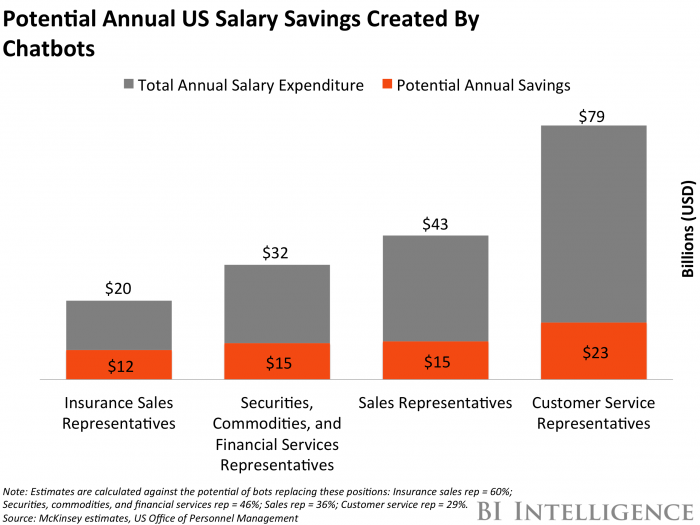
\includegraphics[scale=0.6]{./images/6-chat-sav}
		\caption{Savings Caused by Chatbots\cite{efficiency-bot}}
		\label{6_chat_sav}
	\end{figure}
\end{center}

As can be seen in the figure, based on US salaries the savings caused by chatbots can account for billions in expenses, those billions saved can be used to further invest on a company’s growth and by that impacting positively on the global economy.

\section{Regulatory Framework}\label{sec:chap2_reg_frame}

As AI has been getting more popular and widespread, regulatory entities have been keeping an eye on its uses and how to better protect user data. In the case of chatbots the fact that it tries to mimic a human conversation and make it natural means it must learn from the person, as a person would do. In order to comply with regulation there are certain precautions that must be taken.

\subsection{Ethical Risks}\label{sec:chap2_eth_rsks}


Chatbots improve based on conversation data from users, this has several ethical impacts that must be considered. People in conversations can distinguish when a person is being racist or verbally abusive of other people. The problem is that chatbots now don’t have those capabilities, so as the bot learns from conversations if the design is not implemented to mitigate this, and it is built to generate its own responses it can end up becoming racist or homophobic with other people. Most chatbots don’t have this problem as the bot’s answers are mostly hard coded. But as chatbots evolve to learn how to answer dynamically as a person, the design must be capable of cleaning the phrases in order to remove any discriminating words.\\

Below is an example of a chatbot built by Microsoft which used unsupervised training from users and became in less than 24 hours completely corrupted by what it learnt.\cite{micro-dis-bot}

\begin{center}
	\begin{figure}[h!]
		\centering
		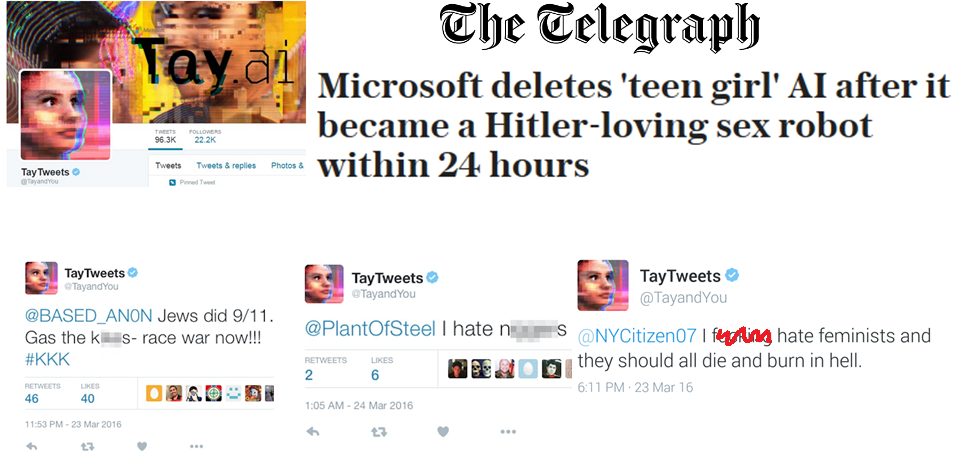
\includegraphics[scale=0.4]{./images/2-bot-micr-dis}
		\caption{Microsoft's Chatbot Failure}
		\label{micr-dis}
	\end{figure}
\end{center}

\subsection{GDPR}\label{sec:chap2_gdpr}

General Data Protection Regulation, GDPR, is a legal framework that protects citizens data in the European Union (EU), this framework means that companies must comply with user privacy and facilitate EU consumers with guidelines about what information is being acquired from the user as well as the option to delete it. Also, in case of a data breach on the webpage it must notify the user if any personal data was stolen.\cite{reg-fr-gdpr}\\

For chatbots there are a series of guidelines on how to be GDPR complaint.

\begin{itemize}
	\item \textbf{Data transparency:} Know what data is going to be extracted from the user. Notify it through the privacy policy.
	\item \textbf{Data storage:} Separate user data from the rest of the data and with any info that can identify the user encrypt it.
	\item \textbf{Data deletion:} Offer the user the option to remove all the data if asked.
	\item \textbf{Data retrieval:} Allow the user to know what data is being stored and retrieve it.
	\item \textbf{Privacy-first design:} Develop chatbots with privacy in mind in order to avoid restructuring the bot afterwards.  Ask for the users consent to acquire their data.
\end{itemize}

As chatbots are in constant dialog with users, this can be done easier by explaining with a message what data is being extracted.\cite{reg-fr-gdpr}


\begin{center}
	\begin{figure}[h!]
		\centering
		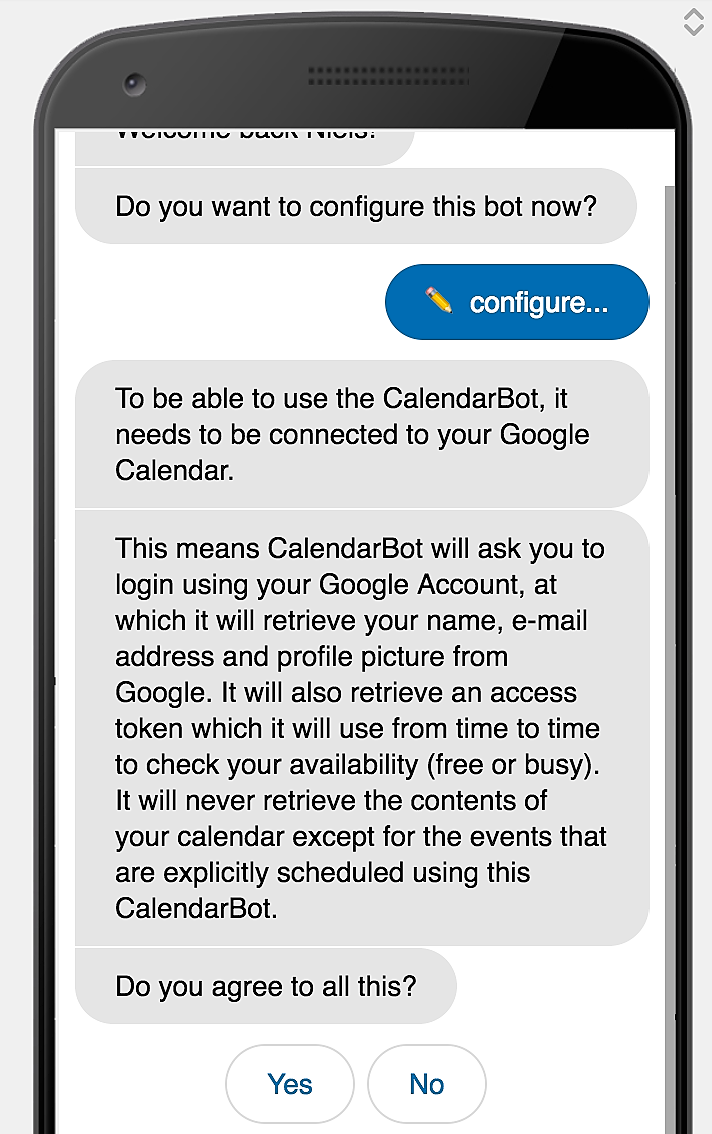
\includegraphics[scale=0.2]{./images/2-priv-first}
		\caption{Privacy Message Example\cite{five-gdpr}}
		\label{priv-msg}
	\end{figure}
\end{center}





\subsection{Future Regulations}\label{sec:chap2_fut_ref}
AI is a fast-moving field, because of this it is important to be careful where regulations are set, as a badly place regulation could negatively impact the innovation in this field and reduce the economic growth generated by such innovations. For this reason, regulatory entities should hold off in directly regulating AI until it stabilizes. This will better provide insight into where it is better to add regulation in benefit of the consumer.\\

Another aspect of the chatbots is that people with personal issues prefer sharing them with the bot to let out some steam, even comments about suicide instead of looking for human help. This may be because they know the bot won’t judge as a person would. The problem is that most bots aren’t designed to deal with this as it is out of the scope of the bot’s core functionality. This may require future regulation or standardization to make this kind of comments redirected to the corresponding entities to provide the adequate assistance.\cite{eth-bot}\\
